% Created by tikzDevice version 0.6.2-92-0ad2792 on 2013-03-04 16:57:09
% !TEX encoding = UTF-8 Unicode
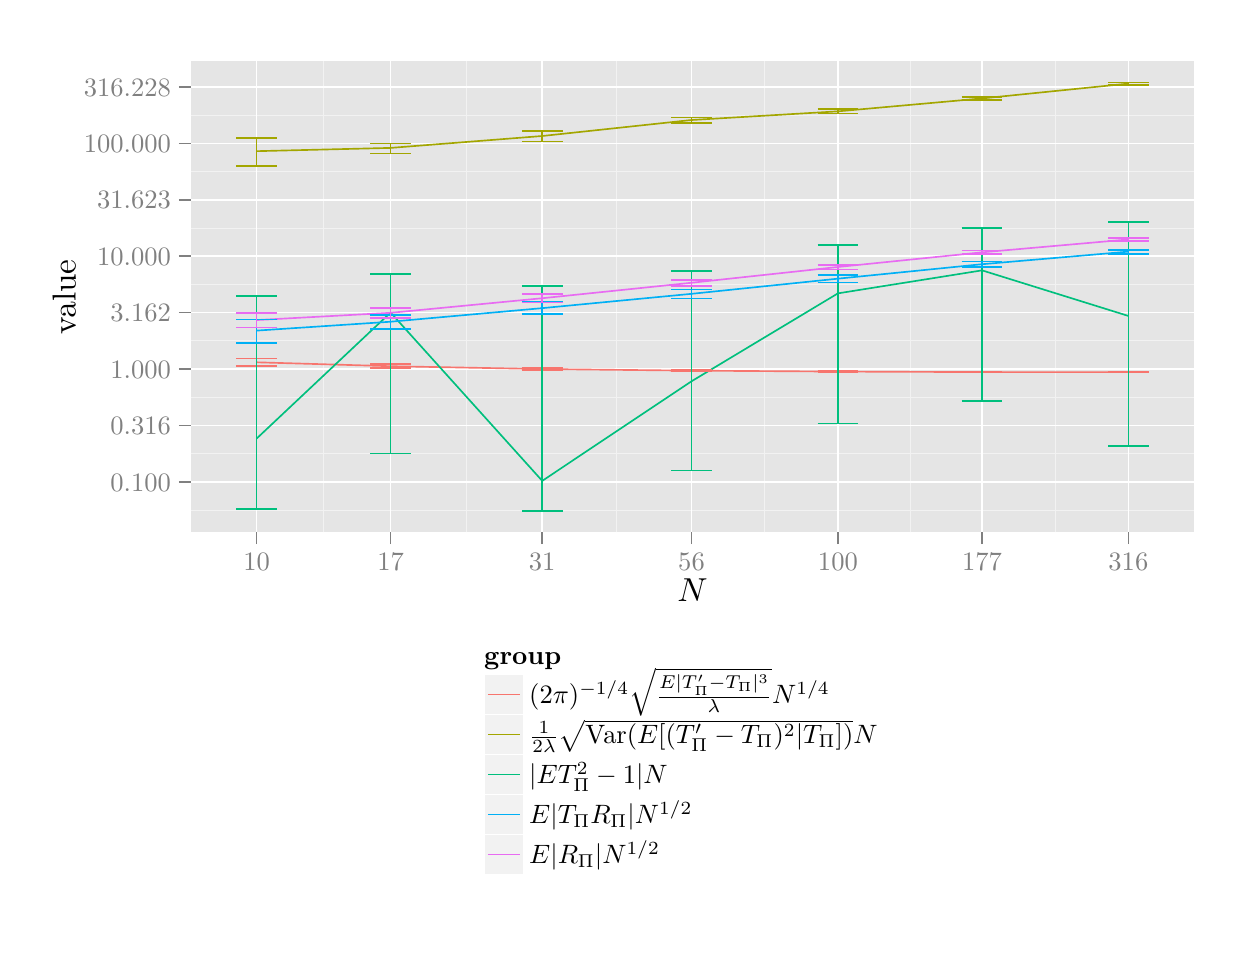
\begin{tikzpicture}[x=1pt,y=1pt]
\definecolor[named]{fillColor}{rgb}{1.00,1.00,1.00}
\path[use as bounding box,fill=fillColor,fill opacity=0.00] (0,0) rectangle (433.62,325.21);
\begin{scope}
\path[clip] (  0.00,  0.00) rectangle (433.62,325.21);
\definecolor[named]{drawColor}{rgb}{1.00,1.00,1.00}
\definecolor[named]{fillColor}{rgb}{1.00,1.00,1.00}

\path[draw=drawColor,line width= 0.6pt,line join=round,line cap=round,fill=fillColor] (  0.00,  0.00) rectangle (433.62,325.21);
\end{scope}
\begin{scope}
\path[clip] ( 58.88,142.81) rectangle (421.57,313.17);
\definecolor[named]{fillColor}{rgb}{0.90,0.90,0.90}

\path[fill=fillColor] ( 58.88,142.81) rectangle (421.57,313.17);
\definecolor[named]{drawColor}{rgb}{0.95,0.95,0.95}

\path[draw=drawColor,line width= 0.3pt,line join=round] ( 58.88,150.87) --
	(421.57,150.87);

\path[draw=drawColor,line width= 0.3pt,line join=round] ( 58.88,171.25) --
	(421.57,171.25);

\path[draw=drawColor,line width= 0.3pt,line join=round] ( 58.88,191.64) --
	(421.57,191.64);

\path[draw=drawColor,line width= 0.3pt,line join=round] ( 58.88,212.03) --
	(421.57,212.03);

\path[draw=drawColor,line width= 0.3pt,line join=round] ( 58.88,232.42) --
	(421.57,232.42);

\path[draw=drawColor,line width= 0.3pt,line join=round] ( 58.88,252.81) --
	(421.57,252.81);

\path[draw=drawColor,line width= 0.3pt,line join=round] ( 58.88,273.20) --
	(421.57,273.20);

\path[draw=drawColor,line width= 0.3pt,line join=round] ( 58.88,293.59) --
	(421.57,293.59);

\path[draw=drawColor,line width= 0.3pt,line join=round] (106.92,142.81) --
	(106.92,313.17);

\path[draw=drawColor,line width= 0.3pt,line join=round] (158.53,142.81) --
	(158.53,313.17);

\path[draw=drawColor,line width= 0.3pt,line join=round] (212.91,142.81) --
	(212.91,313.17);

\path[draw=drawColor,line width= 0.3pt,line join=round] (266.33,142.81) --
	(266.33,313.17);

\path[draw=drawColor,line width= 0.3pt,line join=round] (318.82,142.81) --
	(318.82,313.17);

\path[draw=drawColor,line width= 0.3pt,line join=round] (371.30,142.81) --
	(371.30,313.17);
\definecolor[named]{drawColor}{rgb}{1.00,1.00,1.00}

\path[draw=drawColor,line width= 0.6pt,line join=round] ( 58.88,161.06) --
	(421.57,161.06);

\path[draw=drawColor,line width= 0.6pt,line join=round] ( 58.88,181.44) --
	(421.57,181.44);

\path[draw=drawColor,line width= 0.6pt,line join=round] ( 58.88,201.84) --
	(421.57,201.84);

\path[draw=drawColor,line width= 0.6pt,line join=round] ( 58.88,222.23) --
	(421.57,222.23);

\path[draw=drawColor,line width= 0.6pt,line join=round] ( 58.88,242.62) --
	(421.57,242.62);

\path[draw=drawColor,line width= 0.6pt,line join=round] ( 58.88,263.01) --
	(421.57,263.01);

\path[draw=drawColor,line width= 0.6pt,line join=round] ( 58.88,283.39) --
	(421.57,283.39);

\path[draw=drawColor,line width= 0.6pt,line join=round] ( 58.88,303.78) --
	(421.57,303.78);

\path[draw=drawColor,line width= 0.6pt,line join=round] ( 82.72,142.81) --
	( 82.72,313.17);

\path[draw=drawColor,line width= 0.6pt,line join=round] (131.13,142.81) --
	(131.13,313.17);

\path[draw=drawColor,line width= 0.6pt,line join=round] (185.93,142.81) --
	(185.93,313.17);

\path[draw=drawColor,line width= 0.6pt,line join=round] (239.88,142.81) --
	(239.88,313.17);

\path[draw=drawColor,line width= 0.6pt,line join=round] (292.78,142.81) --
	(292.78,313.17);

\path[draw=drawColor,line width= 0.6pt,line join=round] (344.86,142.81) --
	(344.86,313.17);

\path[draw=drawColor,line width= 0.6pt,line join=round] (397.74,142.81) --
	(397.74,313.17);
\definecolor[named]{drawColor}{rgb}{0.97,0.46,0.43}

\path[draw=drawColor,line width= 0.6pt,line join=round] ( 82.72,204.29) --
	(131.13,202.88) --
	(185.93,201.85) --
	(239.88,201.27) --
	(292.78,200.94) --
	(344.86,200.75) --
	(397.74,200.74);
\definecolor[named]{drawColor}{rgb}{0.64,0.65,0.00}

\path[draw=drawColor,line width= 0.6pt,line join=round] ( 82.72,280.58) --
	(131.13,281.76) --
	(185.93,286.06) --
	(239.88,291.84) --
	(292.78,294.97) --
	(344.86,299.64) --
	(397.74,305.00);
\definecolor[named]{drawColor}{rgb}{0.00,0.75,0.49}

\path[draw=drawColor,line width= 0.6pt,line join=round] ( 82.72,176.72) --
	(131.13,222.28) --
	(185.93,161.45) --
	(239.88,197.43) --
	(292.78,229.20) --
	(344.86,237.51) --
	(397.74,221.04);
\definecolor[named]{drawColor}{rgb}{0.00,0.69,0.96}

\path[draw=drawColor,line width= 0.6pt,line join=round] ( 82.72,215.74) --
	(131.13,218.95) --
	(185.93,223.86) --
	(239.88,229.03) --
	(292.78,234.51) --
	(344.86,239.73) --
	(397.74,244.28);
\definecolor[named]{drawColor}{rgb}{0.91,0.42,0.95}

\path[draw=drawColor,line width= 0.6pt,line join=round] ( 82.72,219.55) --
	(131.13,222.17) --
	(185.93,227.44) --
	(239.88,233.03) --
	(292.78,238.73) --
	(344.86,244.03) --
	(397.74,248.68);
\definecolor[named]{drawColor}{rgb}{0.97,0.46,0.43}

\path[draw=drawColor,line width= 0.6pt,line join=round] ( 75.37,205.63) --
	( 90.07,205.63);

\path[draw=drawColor,line width= 0.6pt,line join=round] ( 82.72,205.63) --
	( 82.72,202.84);

\path[draw=drawColor,line width= 0.6pt,line join=round] ( 75.37,202.84) --
	( 90.07,202.84);

\path[draw=drawColor,line width= 0.6pt,line join=round] (123.78,203.60) --
	(138.48,203.60);

\path[draw=drawColor,line width= 0.6pt,line join=round] (131.13,203.60) --
	(131.13,202.14);

\path[draw=drawColor,line width= 0.6pt,line join=round] (123.78,202.14) --
	(138.48,202.14);

\path[draw=drawColor,line width= 0.6pt,line join=round] (178.58,202.27) --
	(193.28,202.27);

\path[draw=drawColor,line width= 0.6pt,line join=round] (185.93,202.27) --
	(185.93,201.45);

\path[draw=drawColor,line width= 0.6pt,line join=round] (178.58,201.45) --
	(193.28,201.45);

\path[draw=drawColor,line width= 0.6pt,line join=round] (232.53,201.49) --
	(247.23,201.49);

\path[draw=drawColor,line width= 0.6pt,line join=round] (239.88,201.49) --
	(239.88,201.06);

\path[draw=drawColor,line width= 0.6pt,line join=round] (232.53,201.06) --
	(247.23,201.06);

\path[draw=drawColor,line width= 0.6pt,line join=round] (285.42,201.05) --
	(300.13,201.05);

\path[draw=drawColor,line width= 0.6pt,line join=round] (292.78,201.05) --
	(292.78,200.83);

\path[draw=drawColor,line width= 0.6pt,line join=round] (285.42,200.83) --
	(300.13,200.83);

\path[draw=drawColor,line width= 0.6pt,line join=round] (337.51,200.81) --
	(352.22,200.81);

\path[draw=drawColor,line width= 0.6pt,line join=round] (344.86,200.81) --
	(344.86,200.68);

\path[draw=drawColor,line width= 0.6pt,line join=round] (337.51,200.68) --
	(352.22,200.68);

\path[draw=drawColor,line width= 0.6pt,line join=round] (390.39,200.77) --
	(405.09,200.77);

\path[draw=drawColor,line width= 0.6pt,line join=round] (397.74,200.77) --
	(397.74,200.70);

\path[draw=drawColor,line width= 0.6pt,line join=round] (390.39,200.70) --
	(405.09,200.70);
\definecolor[named]{drawColor}{rgb}{0.64,0.65,0.00}

\path[draw=drawColor,line width= 0.6pt,line join=round] ( 75.37,285.23) --
	( 90.07,285.23);

\path[draw=drawColor,line width= 0.6pt,line join=round] ( 82.72,285.23) --
	( 82.72,275.29);

\path[draw=drawColor,line width= 0.6pt,line join=round] ( 75.37,275.29) --
	( 90.07,275.29);

\path[draw=drawColor,line width= 0.6pt,line join=round] (123.78,283.32) --
	(138.48,283.32);

\path[draw=drawColor,line width= 0.6pt,line join=round] (131.13,283.32) --
	(131.13,279.79);

\path[draw=drawColor,line width= 0.6pt,line join=round] (123.78,279.79) --
	(138.48,279.79);

\path[draw=drawColor,line width= 0.6pt,line join=round] (178.58,287.96) --
	(193.28,287.96);

\path[draw=drawColor,line width= 0.6pt,line join=round] (185.93,287.96) --
	(185.93,284.11);

\path[draw=drawColor,line width= 0.6pt,line join=round] (178.58,284.11) --
	(193.28,284.11);

\path[draw=drawColor,line width= 0.6pt,line join=round] (232.53,292.76) --
	(247.23,292.76);

\path[draw=drawColor,line width= 0.6pt,line join=round] (239.88,292.76) --
	(239.88,290.83);

\path[draw=drawColor,line width= 0.6pt,line join=round] (232.53,290.83) --
	(247.23,290.83);

\path[draw=drawColor,line width= 0.6pt,line join=round] (285.42,295.73) --
	(300.13,295.73);

\path[draw=drawColor,line width= 0.6pt,line join=round] (292.78,295.73) --
	(292.78,294.20);

\path[draw=drawColor,line width= 0.6pt,line join=round] (285.42,294.20) --
	(300.13,294.20);

\path[draw=drawColor,line width= 0.6pt,line join=round] (337.51,300.16) --
	(352.22,300.16);

\path[draw=drawColor,line width= 0.6pt,line join=round] (344.86,300.16) --
	(344.86,298.98);

\path[draw=drawColor,line width= 0.6pt,line join=round] (337.51,298.98) --
	(352.22,298.98);

\path[draw=drawColor,line width= 0.6pt,line join=round] (390.39,305.43) --
	(405.09,305.43);

\path[draw=drawColor,line width= 0.6pt,line join=round] (397.74,305.43) --
	(397.74,304.57);

\path[draw=drawColor,line width= 0.6pt,line join=round] (390.39,304.57) --
	(405.09,304.57);
\definecolor[named]{drawColor}{rgb}{0.00,0.75,0.49}

\path[draw=drawColor,line width= 0.6pt,line join=round] ( 75.37,228.34) --
	( 90.07,228.34);

\path[draw=drawColor,line width= 0.6pt,line join=round] ( 82.72,228.34) --
	( 82.72,151.28);

\path[draw=drawColor,line width= 0.6pt,line join=round] ( 75.37,151.28) --
	( 90.07,151.28);

\path[draw=drawColor,line width= 0.6pt,line join=round] (123.78,236.31) --
	(138.48,236.31);

\path[draw=drawColor,line width= 0.6pt,line join=round] (131.13,236.31) --
	(131.13,171.31);

\path[draw=drawColor,line width= 0.6pt,line join=round] (123.78,171.31) --
	(138.48,171.31);

\path[draw=drawColor,line width= 0.6pt,line join=round] (178.58,231.87) --
	(193.28,231.87);

\path[draw=drawColor,line width= 0.6pt,line join=round] (185.93,231.87) --
	(185.93,150.56);

\path[draw=drawColor,line width= 0.6pt,line join=round] (178.58,150.56) --
	(193.28,150.56);

\path[draw=drawColor,line width= 0.6pt,line join=round] (232.53,237.27) --
	(247.23,237.27);

\path[draw=drawColor,line width= 0.6pt,line join=round] (239.88,237.27) --
	(239.88,165.14);

\path[draw=drawColor,line width= 0.6pt,line join=round] (232.53,165.14) --
	(247.23,165.14);

\path[draw=drawColor,line width= 0.6pt,line join=round] (285.42,246.62) --
	(300.13,246.62);

\path[draw=drawColor,line width= 0.6pt,line join=round] (292.78,246.62) --
	(292.78,182.18);

\path[draw=drawColor,line width= 0.6pt,line join=round] (285.42,182.18) --
	(300.13,182.18);

\path[draw=drawColor,line width= 0.6pt,line join=round] (337.51,252.84) --
	(352.22,252.84);

\path[draw=drawColor,line width= 0.6pt,line join=round] (344.86,252.84) --
	(344.86,190.19);

\path[draw=drawColor,line width= 0.6pt,line join=round] (337.51,190.19) --
	(352.22,190.19);

\path[draw=drawColor,line width= 0.6pt,line join=round] (390.39,255.07) --
	(405.09,255.07);

\path[draw=drawColor,line width= 0.6pt,line join=round] (397.74,255.07) --
	(397.74,174.12);

\path[draw=drawColor,line width= 0.6pt,line join=round] (390.39,174.12) --
	(405.09,174.12);
\definecolor[named]{drawColor}{rgb}{0.00,0.69,0.96}

\path[draw=drawColor,line width= 0.6pt,line join=round] ( 75.37,219.70) --
	( 90.07,219.70);

\path[draw=drawColor,line width= 0.6pt,line join=round] ( 82.72,219.70) --
	( 82.72,211.37);

\path[draw=drawColor,line width= 0.6pt,line join=round] ( 75.37,211.37) --
	( 90.07,211.37);

\path[draw=drawColor,line width= 0.6pt,line join=round] (123.78,221.50) --
	(138.48,221.50);

\path[draw=drawColor,line width= 0.6pt,line join=round] (131.13,221.50) --
	(131.13,216.27);

\path[draw=drawColor,line width= 0.6pt,line join=round] (123.78,216.27) --
	(138.48,216.27);

\path[draw=drawColor,line width= 0.6pt,line join=round] (178.58,226.01) --
	(193.28,226.01);

\path[draw=drawColor,line width= 0.6pt,line join=round] (185.93,226.01) --
	(185.93,221.63);

\path[draw=drawColor,line width= 0.6pt,line join=round] (178.58,221.63) --
	(193.28,221.63);

\path[draw=drawColor,line width= 0.6pt,line join=round] (232.53,230.64) --
	(247.23,230.64);

\path[draw=drawColor,line width= 0.6pt,line join=round] (239.88,230.64) --
	(239.88,227.29);

\path[draw=drawColor,line width= 0.6pt,line join=round] (232.53,227.29) --
	(247.23,227.29);

\path[draw=drawColor,line width= 0.6pt,line join=round] (285.42,235.90) --
	(300.13,235.90);

\path[draw=drawColor,line width= 0.6pt,line join=round] (292.78,235.90) --
	(292.78,233.12);

\path[draw=drawColor,line width= 0.6pt,line join=round] (285.42,233.12) --
	(300.13,233.12);

\path[draw=drawColor,line width= 0.6pt,line join=round] (337.51,240.73) --
	(352.22,240.73);

\path[draw=drawColor,line width= 0.6pt,line join=round] (344.86,240.73) --
	(344.86,238.72);

\path[draw=drawColor,line width= 0.6pt,line join=round] (337.51,238.72) --
	(352.22,238.72);

\path[draw=drawColor,line width= 0.6pt,line join=round] (390.39,244.97) --
	(405.09,244.97);

\path[draw=drawColor,line width= 0.6pt,line join=round] (397.74,244.97) --
	(397.74,243.46);

\path[draw=drawColor,line width= 0.6pt,line join=round] (390.39,243.46) --
	(405.09,243.46);
\definecolor[named]{drawColor}{rgb}{0.91,0.42,0.95}

\path[draw=drawColor,line width= 0.6pt,line join=round] ( 75.37,222.00) --
	( 90.07,222.00);

\path[draw=drawColor,line width= 0.6pt,line join=round] ( 82.72,222.00) --
	( 82.72,216.86);

\path[draw=drawColor,line width= 0.6pt,line join=round] ( 75.37,216.86) --
	( 90.07,216.86);

\path[draw=drawColor,line width= 0.6pt,line join=round] (123.78,223.91) --
	(138.48,223.91);

\path[draw=drawColor,line width= 0.6pt,line join=round] (131.13,223.91) --
	(131.13,220.37);

\path[draw=drawColor,line width= 0.6pt,line join=round] (123.78,220.37) --
	(138.48,220.37);

\path[draw=drawColor,line width= 0.6pt,line join=round] (178.58,228.92) --
	(193.28,228.92);

\path[draw=drawColor,line width= 0.6pt,line join=round] (185.93,228.92) --
	(185.93,225.87);

\path[draw=drawColor,line width= 0.6pt,line join=round] (178.58,225.87) --
	(193.28,225.87);

\path[draw=drawColor,line width= 0.6pt,line join=round] (232.53,234.09) --
	(247.23,234.09);

\path[draw=drawColor,line width= 0.6pt,line join=round] (239.88,234.09) --
	(239.88,231.95);

\path[draw=drawColor,line width= 0.6pt,line join=round] (232.53,231.95) --
	(247.23,231.95);

\path[draw=drawColor,line width= 0.6pt,line join=round] (285.42,239.53) --
	(300.13,239.53);

\path[draw=drawColor,line width= 0.6pt,line join=round] (292.78,239.53) --
	(292.78,237.86);

\path[draw=drawColor,line width= 0.6pt,line join=round] (285.42,237.86) --
	(300.13,237.86);

\path[draw=drawColor,line width= 0.6pt,line join=round] (337.51,244.68) --
	(352.22,244.68);

\path[draw=drawColor,line width= 0.6pt,line join=round] (344.86,244.68) --
	(344.86,243.41);

\path[draw=drawColor,line width= 0.6pt,line join=round] (337.51,243.41) --
	(352.22,243.41);

\path[draw=drawColor,line width= 0.6pt,line join=round] (390.39,249.15) --
	(405.09,249.15);

\path[draw=drawColor,line width= 0.6pt,line join=round] (397.74,249.15) --
	(397.74,248.19);

\path[draw=drawColor,line width= 0.6pt,line join=round] (390.39,248.19) --
	(405.09,248.19);
\end{scope}
\begin{scope}
\path[clip] (  0.00,  0.00) rectangle (433.62,325.21);
\definecolor[named]{drawColor}{rgb}{0.50,0.50,0.50}

\node[text=drawColor,anchor=base east,inner sep=0pt, outer sep=0pt, scale=  0.96] at ( 51.77,157.75) {0.100};

\node[text=drawColor,anchor=base east,inner sep=0pt, outer sep=0pt, scale=  0.96] at ( 51.77,178.13) {0.316};

\node[text=drawColor,anchor=base east,inner sep=0pt, outer sep=0pt, scale=  0.96] at ( 51.77,198.53) {1.000};

\node[text=drawColor,anchor=base east,inner sep=0pt, outer sep=0pt, scale=  0.96] at ( 51.77,218.92) {3.162};

\node[text=drawColor,anchor=base east,inner sep=0pt, outer sep=0pt, scale=  0.96] at ( 51.77,239.31) {10.000};

\node[text=drawColor,anchor=base east,inner sep=0pt, outer sep=0pt, scale=  0.96] at ( 51.77,259.70) {31.623};

\node[text=drawColor,anchor=base east,inner sep=0pt, outer sep=0pt, scale=  0.96] at ( 51.77,280.09) {100.000};

\node[text=drawColor,anchor=base east,inner sep=0pt, outer sep=0pt, scale=  0.96] at ( 51.77,300.48) {316.228};
\end{scope}
\begin{scope}
\path[clip] (  0.00,  0.00) rectangle (433.62,325.21);
\definecolor[named]{drawColor}{rgb}{0.50,0.50,0.50}

\path[draw=drawColor,line width= 0.6pt,line join=round] ( 54.61,161.06) --
	( 58.88,161.06);

\path[draw=drawColor,line width= 0.6pt,line join=round] ( 54.61,181.44) --
	( 58.88,181.44);

\path[draw=drawColor,line width= 0.6pt,line join=round] ( 54.61,201.84) --
	( 58.88,201.84);

\path[draw=drawColor,line width= 0.6pt,line join=round] ( 54.61,222.23) --
	( 58.88,222.23);

\path[draw=drawColor,line width= 0.6pt,line join=round] ( 54.61,242.62) --
	( 58.88,242.62);

\path[draw=drawColor,line width= 0.6pt,line join=round] ( 54.61,263.01) --
	( 58.88,263.01);

\path[draw=drawColor,line width= 0.6pt,line join=round] ( 54.61,283.39) --
	( 58.88,283.39);

\path[draw=drawColor,line width= 0.6pt,line join=round] ( 54.61,303.78) --
	( 58.88,303.78);
\end{scope}
\begin{scope}
\path[clip] (  0.00,  0.00) rectangle (433.62,325.21);
\definecolor[named]{drawColor}{rgb}{0.50,0.50,0.50}

\path[draw=drawColor,line width= 0.6pt,line join=round] ( 82.72,138.55) --
	( 82.72,142.81);

\path[draw=drawColor,line width= 0.6pt,line join=round] (131.13,138.55) --
	(131.13,142.81);

\path[draw=drawColor,line width= 0.6pt,line join=round] (185.93,138.55) --
	(185.93,142.81);

\path[draw=drawColor,line width= 0.6pt,line join=round] (239.88,138.55) --
	(239.88,142.81);

\path[draw=drawColor,line width= 0.6pt,line join=round] (292.78,138.55) --
	(292.78,142.81);

\path[draw=drawColor,line width= 0.6pt,line join=round] (344.86,138.55) --
	(344.86,142.81);

\path[draw=drawColor,line width= 0.6pt,line join=round] (397.74,138.55) --
	(397.74,142.81);
\end{scope}
\begin{scope}
\path[clip] (  0.00,  0.00) rectangle (433.62,325.21);
\definecolor[named]{drawColor}{rgb}{0.50,0.50,0.50}

\node[text=drawColor,anchor=base,inner sep=0pt, outer sep=0pt, scale=  0.96] at ( 82.72,129.09) {10};

\node[text=drawColor,anchor=base,inner sep=0pt, outer sep=0pt, scale=  0.96] at (131.13,129.09) {17};

\node[text=drawColor,anchor=base,inner sep=0pt, outer sep=0pt, scale=  0.96] at (185.93,129.09) {31};

\node[text=drawColor,anchor=base,inner sep=0pt, outer sep=0pt, scale=  0.96] at (239.88,129.09) {56};

\node[text=drawColor,anchor=base,inner sep=0pt, outer sep=0pt, scale=  0.96] at (292.78,129.09) {100};

\node[text=drawColor,anchor=base,inner sep=0pt, outer sep=0pt, scale=  0.96] at (344.86,129.09) {177};

\node[text=drawColor,anchor=base,inner sep=0pt, outer sep=0pt, scale=  0.96] at (397.74,129.09) {316};
\end{scope}
\begin{scope}
\path[clip] (  0.00,  0.00) rectangle (433.62,325.21);
\definecolor[named]{drawColor}{rgb}{0.00,0.00,0.00}

\node[text=drawColor,anchor=base,inner sep=0pt, outer sep=0pt, scale=  1.20] at (240.23,117.81) {$N$};
\end{scope}
\begin{scope}
\path[clip] (  0.00,  0.00) rectangle (433.62,325.21);
\definecolor[named]{drawColor}{rgb}{0.00,0.00,0.00}

\node[text=drawColor,rotate= 90.00,anchor=base,inner sep=0pt, outer sep=0pt, scale=  1.20] at ( 17.30,227.99) {value};
\end{scope}
\begin{scope}
\path[clip] (  0.00,  0.00) rectangle (433.62,325.21);
\definecolor[named]{fillColor}{rgb}{1.00,1.00,1.00}

\path[fill=fillColor] (160.71, 14.89) rectangle (319.75,105.93);
\end{scope}
\begin{scope}
\path[clip] (  0.00,  0.00) rectangle (433.62,325.21);
\definecolor[named]{drawColor}{rgb}{0.00,0.00,0.00}

\node[text=drawColor,anchor=base west,inner sep=0pt, outer sep=0pt, scale=  0.96] at (164.98, 95.04) {\bfseries group};
\end{scope}
\begin{scope}
\path[clip] (  0.00,  0.00) rectangle (433.62,325.21);
\definecolor[named]{drawColor}{rgb}{1.00,1.00,1.00}
\definecolor[named]{fillColor}{rgb}{0.95,0.95,0.95}

\path[draw=drawColor,line width= 0.6pt,line join=round,line cap=round,fill=fillColor] (164.98, 76.97) rectangle (179.43, 91.43);
\end{scope}
\begin{scope}
\path[clip] (  0.00,  0.00) rectangle (433.62,325.21);
\definecolor[named]{drawColor}{rgb}{0.97,0.46,0.43}

\path[draw=drawColor,line width= 0.6pt,line join=round] (166.42, 84.20) -- (177.98, 84.20);
\end{scope}
\begin{scope}
\path[clip] (  0.00,  0.00) rectangle (433.62,325.21);
\definecolor[named]{drawColor}{rgb}{0.97,0.46,0.43}

\path[draw=drawColor,line width= 0.6pt,line join=round] (166.42, 84.20) -- (177.98, 84.20);
\end{scope}
\begin{scope}
\path[clip] (  0.00,  0.00) rectangle (433.62,325.21);
\definecolor[named]{drawColor}{rgb}{1.00,1.00,1.00}
\definecolor[named]{fillColor}{rgb}{0.95,0.95,0.95}

\path[draw=drawColor,line width= 0.6pt,line join=round,line cap=round,fill=fillColor] (164.98, 62.52) rectangle (179.43, 76.97);
\end{scope}
\begin{scope}
\path[clip] (  0.00,  0.00) rectangle (433.62,325.21);
\definecolor[named]{drawColor}{rgb}{0.64,0.65,0.00}

\path[draw=drawColor,line width= 0.6pt,line join=round] (166.42, 69.75) -- (177.98, 69.75);
\end{scope}
\begin{scope}
\path[clip] (  0.00,  0.00) rectangle (433.62,325.21);
\definecolor[named]{drawColor}{rgb}{0.64,0.65,0.00}

\path[draw=drawColor,line width= 0.6pt,line join=round] (166.42, 69.75) -- (177.98, 69.75);
\end{scope}
\begin{scope}
\path[clip] (  0.00,  0.00) rectangle (433.62,325.21);
\definecolor[named]{drawColor}{rgb}{1.00,1.00,1.00}
\definecolor[named]{fillColor}{rgb}{0.95,0.95,0.95}

\path[draw=drawColor,line width= 0.6pt,line join=round,line cap=round,fill=fillColor] (164.98, 48.07) rectangle (179.43, 62.52);
\end{scope}
\begin{scope}
\path[clip] (  0.00,  0.00) rectangle (433.62,325.21);
\definecolor[named]{drawColor}{rgb}{0.00,0.75,0.49}

\path[draw=drawColor,line width= 0.6pt,line join=round] (166.42, 55.29) -- (177.98, 55.29);
\end{scope}
\begin{scope}
\path[clip] (  0.00,  0.00) rectangle (433.62,325.21);
\definecolor[named]{drawColor}{rgb}{0.00,0.75,0.49}

\path[draw=drawColor,line width= 0.6pt,line join=round] (166.42, 55.29) -- (177.98, 55.29);
\end{scope}
\begin{scope}
\path[clip] (  0.00,  0.00) rectangle (433.62,325.21);
\definecolor[named]{drawColor}{rgb}{1.00,1.00,1.00}
\definecolor[named]{fillColor}{rgb}{0.95,0.95,0.95}

\path[draw=drawColor,line width= 0.6pt,line join=round,line cap=round,fill=fillColor] (164.98, 33.61) rectangle (179.43, 48.07);
\end{scope}
\begin{scope}
\path[clip] (  0.00,  0.00) rectangle (433.62,325.21);
\definecolor[named]{drawColor}{rgb}{0.00,0.69,0.96}

\path[draw=drawColor,line width= 0.6pt,line join=round] (166.42, 40.84) -- (177.98, 40.84);
\end{scope}
\begin{scope}
\path[clip] (  0.00,  0.00) rectangle (433.62,325.21);
\definecolor[named]{drawColor}{rgb}{0.00,0.69,0.96}

\path[draw=drawColor,line width= 0.6pt,line join=round] (166.42, 40.84) -- (177.98, 40.84);
\end{scope}
\begin{scope}
\path[clip] (  0.00,  0.00) rectangle (433.62,325.21);
\definecolor[named]{drawColor}{rgb}{1.00,1.00,1.00}
\definecolor[named]{fillColor}{rgb}{0.95,0.95,0.95}

\path[draw=drawColor,line width= 0.6pt,line join=round,line cap=round,fill=fillColor] (164.98, 19.16) rectangle (179.43, 33.61);
\end{scope}
\begin{scope}
\path[clip] (  0.00,  0.00) rectangle (433.62,325.21);
\definecolor[named]{drawColor}{rgb}{0.91,0.42,0.95}

\path[draw=drawColor,line width= 0.6pt,line join=round] (166.42, 26.39) -- (177.98, 26.39);
\end{scope}
\begin{scope}
\path[clip] (  0.00,  0.00) rectangle (433.62,325.21);
\definecolor[named]{drawColor}{rgb}{0.91,0.42,0.95}

\path[draw=drawColor,line width= 0.6pt,line join=round] (166.42, 26.39) -- (177.98, 26.39);
\end{scope}
\begin{scope}
\path[clip] (  0.00,  0.00) rectangle (433.62,325.21);
\definecolor[named]{drawColor}{rgb}{0.00,0.00,0.00}

\node[text=drawColor,anchor=base west,inner sep=0pt, outer sep=0pt, scale=  0.96] at (181.24, 80.90) {$(2\pi)^{-1/4}\sqrt{\frac{\mathbb{E}|T'_{\Pi}-T_{\Pi}|^3}{\lambda}}N^{1/4}\quad $};
\end{scope}
\begin{scope}
\path[clip] (  0.00,  0.00) rectangle (433.62,325.21);
\definecolor[named]{drawColor}{rgb}{0.00,0.00,0.00}

\node[text=drawColor,anchor=base west,inner sep=0pt, outer sep=0pt, scale=  0.96] at (181.24, 66.44) {$\frac{1}{2\lambda}\sqrt{\mathrm{Var}(\mathbb{E}[(T'_{\Pi}-T_{\Pi})^2|T_{\Pi}])}N\quad $};
\end{scope}
\begin{scope}
\path[clip] (  0.00,  0.00) rectangle (433.62,325.21);
\definecolor[named]{drawColor}{rgb}{0.00,0.00,0.00}

\node[text=drawColor,anchor=base west,inner sep=0pt, outer sep=0pt, scale=  0.96] at (181.24, 51.99) {$|\mathbb{E}T_{\Pi}^2-1|N\quad $};
\end{scope}
\begin{scope}
\path[clip] (  0.00,  0.00) rectangle (433.62,325.21);
\definecolor[named]{drawColor}{rgb}{0.00,0.00,0.00}

\node[text=drawColor,anchor=base west,inner sep=0pt, outer sep=0pt, scale=  0.96] at (181.24, 37.53) {$\mathbb{E}|T_{\Pi}R_{\Pi}|N^{1/2}\quad $};
\end{scope}
\begin{scope}
\path[clip] (  0.00,  0.00) rectangle (433.62,325.21);
\definecolor[named]{drawColor}{rgb}{0.00,0.00,0.00}

\node[text=drawColor,anchor=base west,inner sep=0pt, outer sep=0pt, scale=  0.96] at (181.24, 23.08) {$\mathbb{E}|R_{\Pi}|N^{1/2}\quad $};
\end{scope}
\end{tikzpicture}
